\documentclass[border=3mm]{standalone}

\usepackage{tikz}
\usetikzlibrary{decorations.markings,arrows.meta}

\begin{document}
	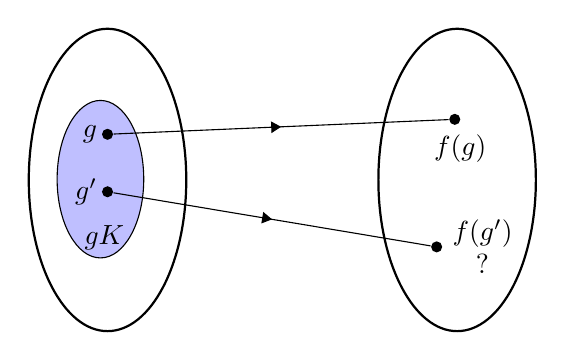
\begin{tikzpicture}
		\draw[thick]  (-2.13,-0.12) ellipse (1 and 1.92);
		\draw[thick]  (2.31,-0.12) ellipse (1 and 1.92);
		\draw[fill=blue!25]  (-2.22,-0.11) ellipse (0.55 and 1.);
		\node[circle,fill=black,inner sep=0pt,minimum size=4pt,label={left,xshift=2pt:$g$}] (1) at (-2.13,0.46) {};
		\node[circle,fill=black,inner sep=0pt,minimum size=4pt,label={below,xshift=2pt:$f(g)$}] (2) at (2.28,0.65) {};
		\node[circle,fill=black,inner sep=0pt,minimum size=4pt,label={ left,xshift=2pt:$g'$}] (3) at (-2.13,-0.27) {};
		\node[circle,fill=black,inner sep=0pt,minimum size=4pt,label={right,align=center:$f(g')$\\?}] (4) at (2.05,-0.97) {};
		\node at (-2.17,-0.85) {$gK$};
	\begin{scope}[decoration={
		markings,
		mark=at position 0.5 with {\arrow{Triangle}}
	}]
		\draw[postaction={decorate}] (1) -- (2);
		\draw[postaction={decorate}] (3) -- (4);
	\end{scope}
	\end{tikzpicture}
\end{document}